%% LaTeX template for the science justification & technical
%% feasibility to be submitted as part of a TESS Guest Investigator
%% Program proposal. This template is based on the proposal template
%% used by the NuSTAR mission.
%%
%% TESS Guest Investigator Proposal Cycle 1 template
%% V1.0
%% 2017-08-04


%%%%%%%%%%%%%%%%%%%%%%%%%%%
%%%%% DOCUMENT FORMAT %%%%%
%%%%%%%%%%%%%%%%%%%%%%%%%%%

%% The default font was chosen to be easily readable while allowing
%% sufficient material to be included.

%% Please note that the proposal will be printed on US Letter size paper,
%% 8.5 in x 11 in, and that formatting the text for other sizes will
%% generally cause layout problems and may result in text being cut
%% off near the edges. PLEASE DO NOT CHANGE THE 'LETTERPAPER' OPTION
%% IN THE DOCUMENTCLASS COMMAND.

%%%%%%%%%%%%%%%%%%%%%%%%%%%%%%%%%%%%%%%%%%%%%%
%%%%% Default format: 11pt single column %%%%%
%%%%%%%%%%%%%%%%%%%%%%%%%%%%%%%%%%%%%%%%%%%%%%

%% NOTE: NASA ROSES requires body font size to be no smaller than 15 
%% characters per inch (equivalent to Times Roman 12 point).
%%
%% Minimum margin size is 1 inch from top, bottom, and sides.

\documentclass[letterpaper,11pt]{article}

%%%%%%%%%%%%%%%%%%%%%%%%%%%%%%%%%%
%%%%% HOW TO INCLUDE FIGURES %%%%%
%%%%%%%%%%%%%%%%%%%%%%%%%%%%%%%%%%

%% Please see the ``Included packages'' section below.

%%%%%%%%%%%%%%%%%%%%%%%%%%%%%
%%%%% Included packages %%%%%
%%%%%%%%%%%%%%%%%%%%%%%%%%%%%

\usepackage{graphics,graphicx}
\usepackage{hyperref}
\usepackage{caption}
\usepackage{subcaption}
\usepackage{comment}
\usepackage{amssymb}
\usepackage{setspace}
\renewcommand{\baselinestretch}{1.0} 


%\usepackage[colorlinks]{hyperref}
%\hypersetup{urlcolor=blue}
%\usepackage{cleveref}

\usepackage{natbib}
\usepackage{bibentry} %needed for "nobibliography" option
% abbrvnat, modded to fix length of references, and to not show title
\bibliographystyle{abbrvnat86}
\setcitestyle{authoryear,open={(},close={)}}
\setlength{\bibsep}{0pt plus 0.2ex} % set bibliography line separation small
\renewcommand{\bibsection}{} % get rid of "References" heading

%% Feel free to modify the included packages list to use your
%% favorite packages. 

%% In the graphics and graphicx packages, Postscript and eps figures
%% can be included using the \includegraphics command. The graphics
%% package is part of standard LaTeX2e and provides a basic way of including a
%% figure. The graphicx package is not standard, but extends the
%% \includegraphics command to make it more user-friendly. If graphicx
%% is not available on your system please remove it from the list of
%% included packages above.  

%% Syntax:
%% In the graphics package:
%%
%% \begin{figure}
%% \includegraphics[llx,lly][urx,ury]{file}
%% \end{figure}
%%
%% where ll denotes 'lower left' and ur 'upper right' and the x and y
%% values are the coordinates of the PostScript bounding box in
%% points. There are 72 points in an inch.
%%
%% In the graphicx package:
%% 
%% \begin{figure}
%% \includegraphics[key=val,key=val,...]{file}
%% \end{figure}
%%
%% where some of the useful keys are: angle, width, height,
%% keepaspectratio (='true' or 'false') and scale. Bounding box values
%% can be given as [bb=llx lly urx ury].
%%
%% In either case you have to use LaTeX figure placement commands to
%% position the figure on the page; \includegraphics will not do
%% that. Both these commands also have other options that are listed
%% in the LaTeX manual (for the graphics package) and in 'The LaTeX
%% Graphics Companion' (for the graphicx package).



%%%%%%%%%%%%%%%%%%%%%%%%%%%
%%%%% Page dimensions %%%%%
%%%%%%%%%%%%%%%%%%%%%%%%%%%

\setlength{\textwidth}{6.5in} 
\setlength{\textheight}{9in}
\setlength{\topmargin}{-0.0625in} 
\setlength{\oddsidemargin}{0in}
\setlength{\evensidemargin}{0in} 
\setlength{\headheight}{0in}
\setlength{\headsep}{0in} 
\setlength{\hoffset}{0in}
\setlength{\voffset}{0in}
\setlength{\skip\footins}{2ex}

% remove excess white space
\setlength\belowcaptionskip{-3ex}


%%%%%%%%%%%%%%%%%%%%%%%%%%%%%%%%%%
%%%%% Section heading format %%%%%
%%%%%%%%%%%%%%%%%%%%%%%%%%%%%%%%%%

\makeatletter
\renewcommand\section{\@startsection%
{section}{1}{0mm}{-0.5\baselineskip}%
{0.5\baselineskip}{\normalfont\normalsize\bfseries}}%
\makeatother

%%%%%%%%%%%%%%%%%%%%%%%%%%%%%%%%%%%%%
%%%%% Some Useful Abbreviations %%%%% 
%%%%%%%%%%%%%%%%%%%%%%%%%%%%%%%%%%%%%
\newcommand{\tess}{{\it TESS}}
\newcommand{\jwst}{{\it JWST}}
\newcommand{\kepler}{{\it Kepler}}
\newcommand{\ktwo}{{\it K2}}
\newcommand{\hst}{{\it HST}}
\newcommand{\msun}{$M_{\odot}$}
\newcommand{\rsun}{$R_{\odot}$}
\newcommand{\lsun}{$L_{\odot}$}
\newcommand{\re}{$R_{\oplus}$}
\newcommand{\me}{$M_{\oplus}$}
\newcommand{\rj}{$R_{\textrm{\scriptsize Jup}}$}
\newcommand{\mj}{$M_{\textrm{\scriptsize Jup}}$}
\newcommand{\ms}{m~s$^{-1}$}



%%%%%%%%%%%%%%%%%%%%%%%%%%%%%
%%%%% Start of document %%%%% 
%%%%%%%%%%%%%%%%%%%%%%%%%%%%%

\begin{document}
%\nobibliography{bibliography}{}
\pagestyle{plain}
\pagenumbering{arabic}


 
%%%%%%%%%%%%%%%%%%%%%%%%%%%%%
%%%%% Title of proposal %%%%% 
%%%%%%%%%%%%%%%%%%%%%%%%%%%%%

\begin{center} 
\bfseries\uppercase{
  Difference Imaging Makes A Difference: Probing Exoplanet Age Evolution With 
All-Sky Cluster Surveys  
}
\end{center}



%%%%%%%%%%%%%%%%%%%%%%%%%%%%%%%%%%%%%%%%%
%%%%% Body of science justification %%%%%
%%%%% and technical feasibility     %%%%%
%%%%%%%%%%%%%%%%%%%%%%%%%%%%%%%%%%%%%%%%%


\vspace{-4mm}






\section{Scientific Motivation}

\vspace{-0.3mm}
Each of the $\sim$1000 star clusters of the Milky Way is a gift to
astrophysics, providing a sample of stars that vary widely in mass
but all have approximately the same age and composition.  Time-series
photometry of clusters\footnote{For brevity, we use this term to refer
  to open clusters, moving groups, associations, and star-forming
  regions.} has numerous applications.  By measuring rotation periods
over a range of ages, we can study the angular momentum evolution of
stars and improve our ability to determine stellar ages through
``gyrochronology.'' By measuring eccentricities as a function age, we
can study the tidal evolution of binaries. The detection of eclipsing
binaries can lead to the precise determination of the absolute
dimensions of the stars and stringent tests of stellar-evolutionary
models.  Circumstellar material can also be studied by finding the
rare cases in which the material produces eclipses.

The detection of transiting planets --- our main motivation for the
proposed work --- will shed light on the timescales for processes in
planet formation, evolution, and migration, and on the effects of
cluster density. With a larger sample of transiting planets in clusters of
varying ages, we could see the evolution of the radius distribution of
giant planets as they contract \citep{Fortney_et_al_2007}, and watch
as the closest-in planets lose mass to photo-evaporation
\citep{Owen_Wu_2017, Fulton_et_al_2017}.  The Hyades planet K2-25b
\citep{Mann_K2_25_2016}, for example, appears to be oversized compared
to mature planets of the same mass and irradiation.  By searching for
hot Jupiters in clusters we can determine when these misplaced planes
begin to appear,
thereby constraining theories for their formation. The discovery of
K2-33b has already showed that in at least one case a hot Neptune was
able to form in fewer than 10~Myr \citep{David_et_al_2017,Mann_K2_33b_2016}.
Detecting planets in dense clusters ($\gtrsim$1000\,pc$^{-3}$) may
also reveal how the stellar encounters affect planetary
system architecture \citep{Meibom_et_al_2013}.  Yet most of this work
remains for the future: only about 10 of the currently known
transiting planets are in clusters.

In mid-2018, the Transiting Exoplanet Survey Satellite (\tess) will
begin searching for exoplanets.  The mission's main
goal is to detect small transiting planets around bright stars, and to
measure their masses using ground-based Doppler spectroscopy.  Within a
few months of data acquisition, the {\it TESS} team will release light curves
with 2-minute sampling for a few hundred thousand pre-selected target
stars.  These target stars will be chosen based on planet
detectability~\citep{Stassun_et_al_2017}.  In addition, the mission will
release full-frame images with 30-minute sampling, which are a ``bonus''
that were not part of the original mission goals.

Through its full-frame images, \tess\ holds the promise to
deliver the most homogeneous and comprehensive photometric cluster
survey in history.  Based on the cluster membership database of
\citet{Kharchenko_et_al_2013} and the $\!$\tess\ apparent magnitude
calculator of~\citet{Jaffe_Barclay_2017}, we estimate that $10^5$
cluster members brighter than $T=16$ will be observed in each
ecliptic hemisphere's full-frame images.

There will be formidable obstacles to deriving precise
photometry from {\it TESS} images of cluster fields because
of the relatively poor angular resolution ($\approx 20''/{\rm px}$).
Almost all clusters are within 10 degrees of the Galactic
plane (see Figure~\ref{fig:cluster_positions_dilution}),
where the problems with crowding and complex backgrounds are so severe that 
the {\it TESS}\,
Science Team has neglected that portion of the sky in their planet
simulations \citep{Sullivan_et_al_2015}. 
Similarly, the {\it TESS}\, target star list deprioritizes all objects 
within $15^\circ$ of the galactic plane~\citep{Stassun_et_al_2017}, which 
includes 90\% of
all star clusters.  The large pixel size and the high stellar surface
density will make aperture photometry unreliable.  Yet,
aperture photometry is the basis of the official {\it TESS} data
reduction pipeline and almost all reduction methods that have been
applied to {\it Kepler} and {\it K2} data.

These challenges are substantial --- and surmountable, with the tools
that have been used to analyze ground-based images with very similar 
characteristics to those of {\it TESS} images.  {\bf We
  propose to produce light curves of star cluster members by applying
  difference-imaging methods to the {\it TESS} full-frame images.}
Our own motivation is to search for transiting giant planets, but we will 
deliver these light curves promptly to the MAST public archive
for the entire community to perform a wide range of scientific
investigations.

\begin{figure}[!tb]
    \begin{subfigure}{.6\textwidth}
        \centering
        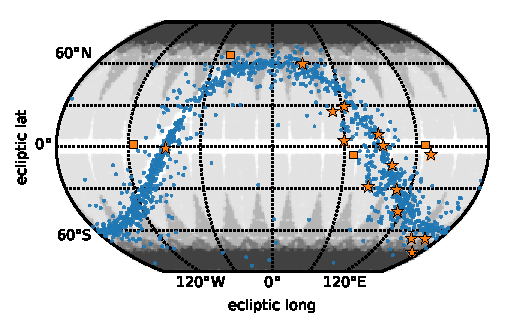
\includegraphics[width=1.02\textwidth]{figures/cluster_positions_ecliptic_scicase.pdf}
        %\caption{A subfigure}
        %\label{fig:sub2}
    \end{subfigure}
    \begin{subfigure}{.4\textwidth}
        \centering
        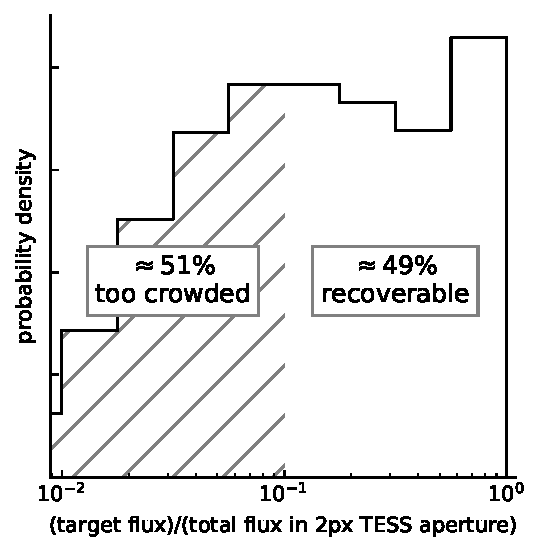
\includegraphics[width=.95\textwidth]{figures/dil_Tmaglt16_dlt2kpc_members.pdf}
        %\caption{A subfigure}
        %\label{fig:sub3}
    \end{subfigure}
    \caption{ {\it Left:\,} Clusters are at low galactic latitudes. Each
      ecliptic hemisphere has about $10^5$ cluster stars with
      $T<16$ and $d < 2\,{\rm kpc}$. Blue circles show 885
      documented clusters \citep{Kharchenko_et_al_2013}. Orange stars are the
      clusters that have been closely monitored by ground-based telescopes. 
      Orange squares are clusters that were surveyed by \kepler\ and \ktwo.
      {\it TESS} will provide homogeneous and continuous data for most of 
      these clusters (shaded background).  
    \newline{\it Right:} The dilution problem. Within a standard
    aperture, a single cluster star usually contributes only a small
    fraction of the total flux. Shown here is the histogram of this
    flux fraction for cluster stars with $T<16$ and $d<2\,{\rm
      kpc}$. Almost none are well suited to aperture photometry. About
    half have flux fractions $>0.1$ and will be amenable to difference
    imaging. 
    \label{fig:cluster_positions_dilution}
    }
\end{figure}

\vspace{-0.3mm}
\section{Team \& Context}
\vspace{-0.3mm}

Ph.D. student Luke Bouma will hold primary responsibility for the project.
Mr.$\ $Bouma will process the \tess\ full-frame images, produce light curves, 
and deliver them to the MAST archive. He will search the light curves for 
transiting exoplanets, oversee follow-up observations of candidates, and lead 
the subsequent analysis effort.
This will be accomplished under the supervision of Prof.$\ $Joshua Winn (PI), 
and collaborating with Prof.$\ $G\'asp\'ar Bakos, Dr.$\ $Joel Hartman, and 
Dr.$\ $Waqas Bhatti.

Our group has extensive experience with precise time-series
photometry, including difference imaging and cluster photometry,
through our leadership of the HATNet and HATSouth transiting planet
surveys as well as deep surveys of crowded fields in M\,37 and 
M\,33~\citep{hartman_deep_2006,hartman_deep_2009}.  We are commissioning a new
multi-telescope observatory called HATPI, at Las Campanas Observatory,
employing 63 wide-field 10~cm lenses that have a pixel scale similar
to the {\it TESS} cameras. 
The combined HATPI, HATSouth, and HATNet datasets will compliment
\tess, and will help in discovering large planets with only a few transits in 
the $28\,{\rm days}$ of \tess\ photometry.

\vspace{-0.3mm}
\section{Data Reduction Plan}
\vspace{-0.3mm}

The concept of difference imaging (also called image subtraction) is
to isolate variable sources from within blends and complex
backgrounds, by subtracting each image from an appropriate convolution
of a master image \citep{Alard_Lupton_1998}. 

We have an existing software pipeline for difference imaging, photometry, and 
detrending. Our implementation is a descendant of the \texttt{fitsh} code, 
described by~\citet{Pal_2012}. Our light curve processing tools are based on
\texttt{VARTOOLS}~\citep{Hartman_Bakos_2016} and 
\texttt{astrobase}~\citep{bhatti_astrobase_2018}.
We also have modules for filtering instrumental systematics from 
the light curves, leaving only astrophysical 
signals~~\citep{Kovacs_et_al_2005,Bakos_et_al_2010}.
Our tools for identification and vetting of candidate transit signals are 
well-tested: they have been honed over 15 years and more than 100 planet 
discoveries.
We also successfully applied our pipeline to {\it K2} data.
In a project led by a Princeton Ph.D. student,
\citet{Soares-Furtado_et_al_2017} performed difference imaging on a
\ktwo\ ``superstamp'' covering the open clusters M\,35 and NGC\,2158,
leading to the most precise time-series photometry that is currently
available for those fields.

Figure~\ref{fig:hatpi_feasibile} shows that our image subtraction
pipeline can successfully reduce HATPI images, which will be very
similar to \tess\ full-frame images.  
Mr.$\ $Bouma will reduce and analyze three years of 
similar data from the HATPI prototype instrument before the initial \tess\ 
data release, which will provide an opportunity for further software testing.

\begin{figure}[!t]
    \centering
    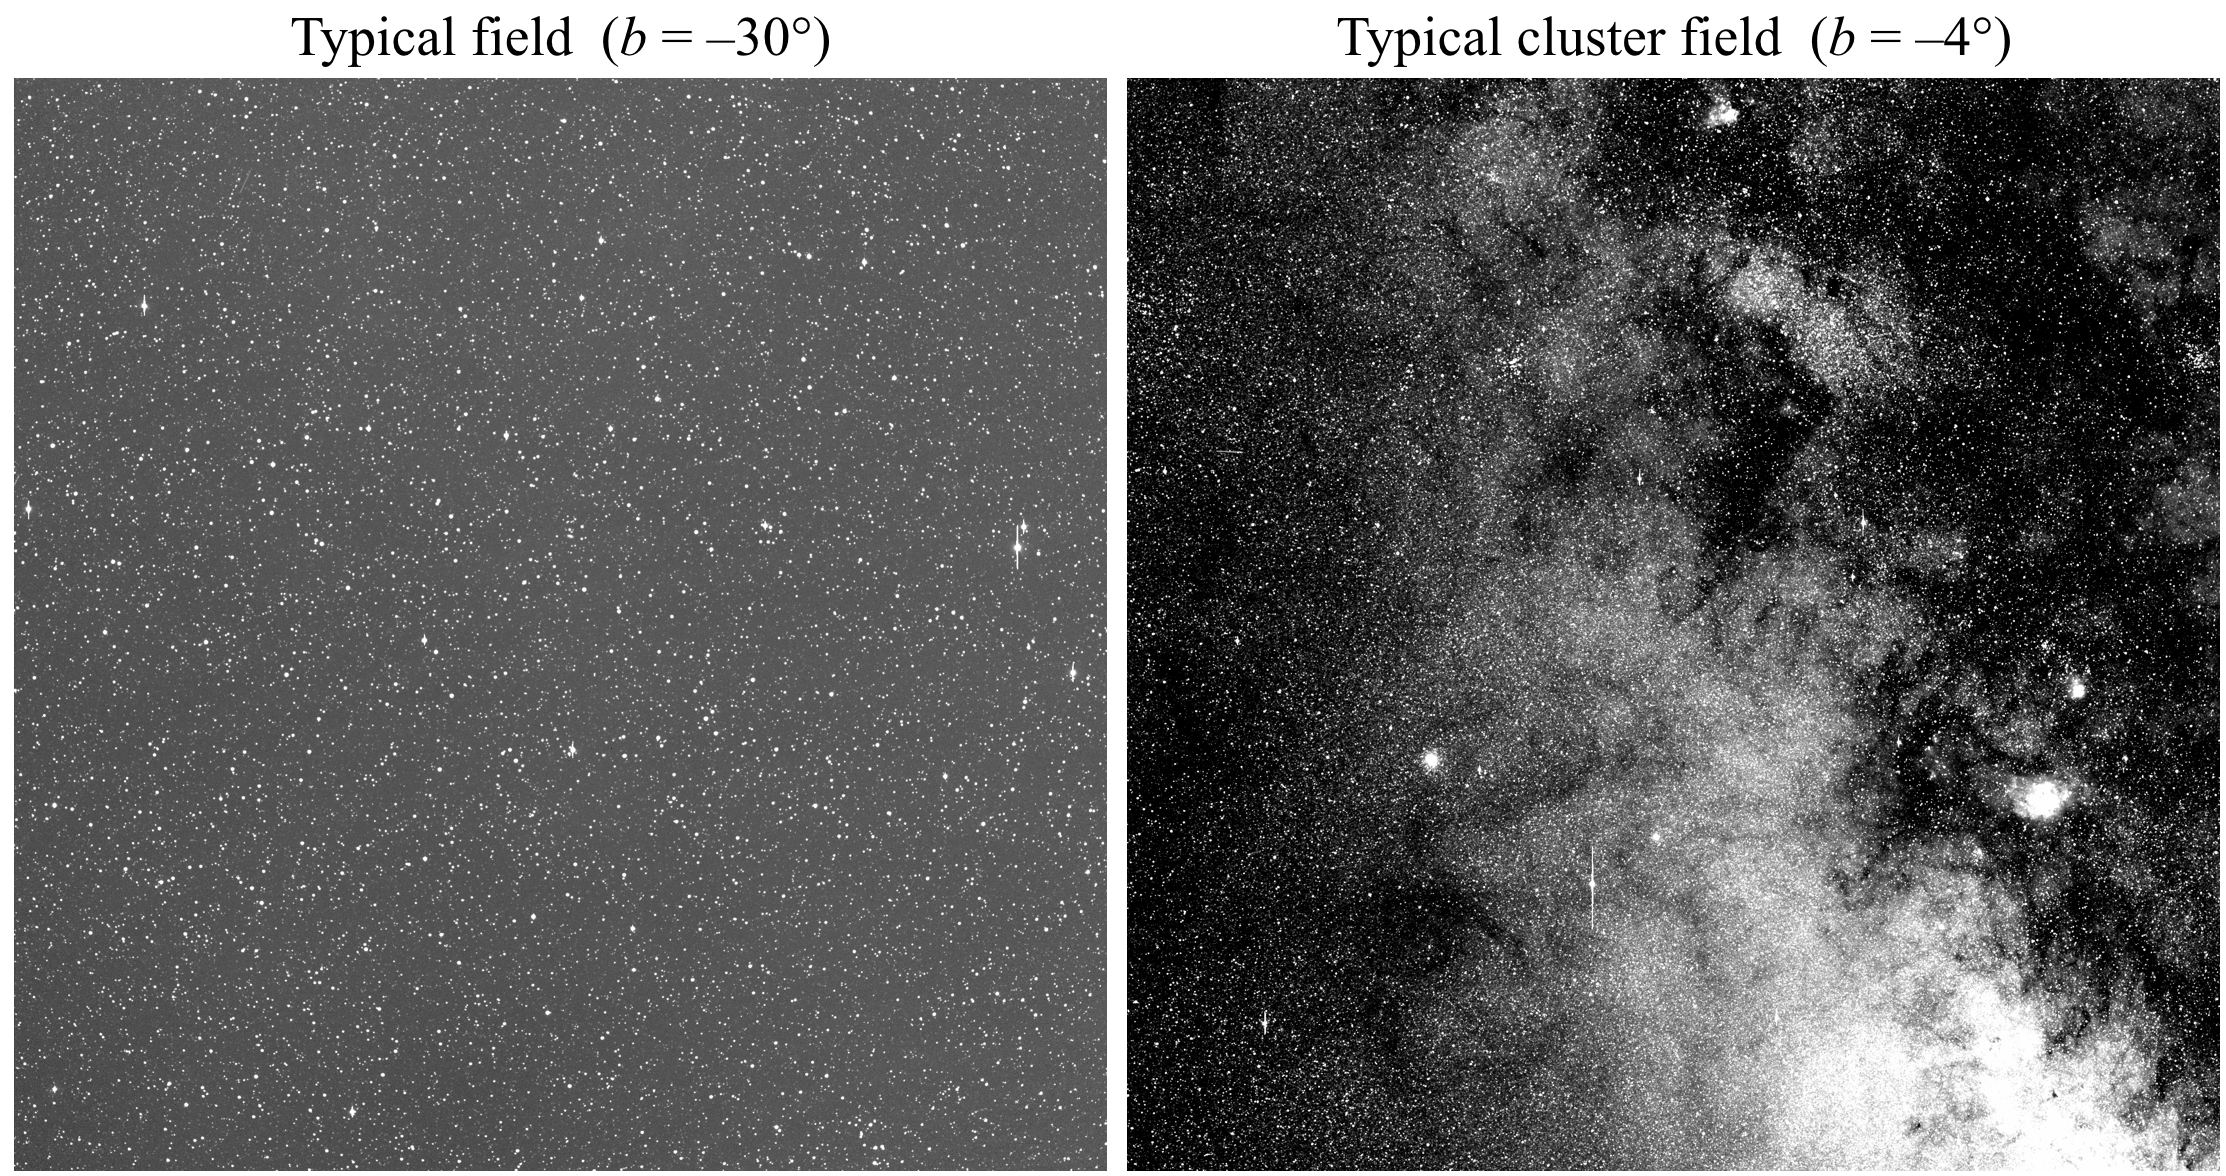
\includegraphics[width=.85\textwidth]{figures/FieldComparison.png}
    \caption{The problem of crowding. Each field is a real 13$^\circ$ image
      from HATPI, which has nearly the same pixel scale as {\it TESS}. On the 
      left
      is a typical field, for which aperture photometry will be adequate.
      On the right is a typical {\it cluster} field, for which aperture 
      photometry
      cannot be relied upon. Difference imaging is required to isolate
      sources of photometric variability.
      \label{fig:FieldComparison}}
\end{figure}

\vspace{-0.3mm}
\section{Necessity and Feasibility}
\label{sec:technical_feasibility}
\vspace{-0.3mm}

For almost all the clusters {\it TESS} will observe, image subtraction
is necessary to produce reliable light curves.  One way to quantify
the blending problem is to ask what fraction of the total flux in a
photometric aperture is contributed by a particular target star.
Aperture photometry is reliable when this fraction is close to unity.
Difference imaging, in our experience, can produce reliable photometry
even when this fraction is as low as 0.1.  Based on the cluster
membership data of \citet{Kharchenko_et_al_2013}, and the density of
background stars, we find that the median dilution fraction of stars
with $T<16$ is 0.13 for an aperture radius of 2 pixels. Difference
imaging is therefore essential, and feasible.

As noted above, the scope of scientific investigations that will be
possible with cluster light curves is very broad.  Since our own
interest is in transiting planets, we have assessed the prospects for
planet detection in the following manner.  We used the {\it TESS}
noise model of \citet{Sullivan_et_al_2015}, as implemented in the code
of \citet{Jaffe_Barclay_2017}, to predict the achievable noise
level for all $T<16$ cluster members in the southern ecliptic
hemisphere.  Using the catalog values of the color and age of each
star, we estimated the mass and radius with reference to the
stellar-evolutionary models of \citet{Siess_et_al_2000}. We then
calculated the number of stars for which a planet with a 10-day period
could be detected with a signal-to-noise ratio exceeding 10, even in
the face of the estimated flux dilution.

During \tess\ Cycle 1 ($\sim$June 2018-2019) we find that 20,000 cluster stars 
can be searched for Jupiter-sized planets, and 3,200 stars can be searched for
Neptune-sized planets.  Taking into account the transit probability,
and a typical occurrence of 0.5\%, this would result in about 15 hot
Jupiters and 5 hot Neptunes.  To put this into perspective, there are
currently only 13 transiting cluster planets known, and only one transiting hot
Jupiter \citep{David_et_al_2017,Mann_et_al_2017}.
\tess\ will observe a comparable number of cluster stars in Cycle 2 
($\sim$June 2019-2020), which will double the yields, giving a total of 30 hot 
Jupiters and 10 hot Neptunes by the end of \tess\ Cycle~2.

We will follow up planet candidates through our participation in the {\it TESS}
Follow-up Observing Program and the international KESPRINT consortium.
We also have 100\% of the observing time on the newly deployed CHAT
0.7$\,$m automated photometric telescope at Las Campanas Observatory,
Chile. Dedicated observations with CHAT will allow us to obtain images with 
better photometric precision and higher spatial resolution ($\approx 
0.7''/{\rm px}$) than {\it TESS}. This will be essential in helping us
determine which star is responsible for transits in heavily blended regions of 
clusters.
The HATNet and HATSouth teams have many years of experience vetting transit 
candidates, and have confirmed over 100 transiting planets from their combined 
surveys.

\vspace{-0.3mm}
\section{Expected Impact}
\label{sec:impact}

\vspace{-0.3mm}
\begin{figure}[!t]
    \centering
    \begin{subfigure}{.333\textwidth}
        \centering
        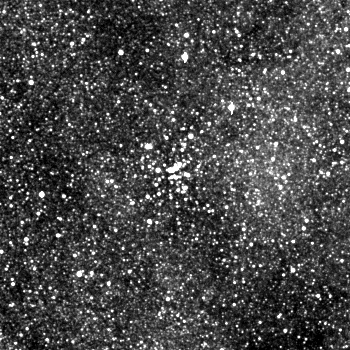
\includegraphics[width=.99\textwidth]{figures/M25_crop.png}
        %\caption{A subfigure}
        %\label{fig:sub1}
    \end{subfigure}%
    \begin{subfigure}{.333\textwidth}
        \centering
        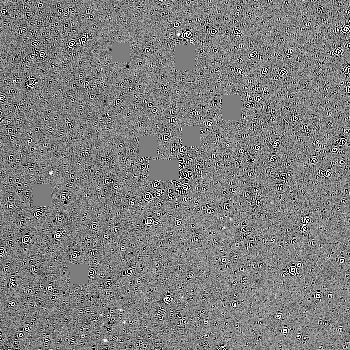
\includegraphics[width=.99\textwidth]{figures/M25_sub_crop.png}
        %\caption{A subfigure}
        %\label{fig:sub2}
    \end{subfigure}
    \begin{subfigure}{.30\textwidth}
        \centering
        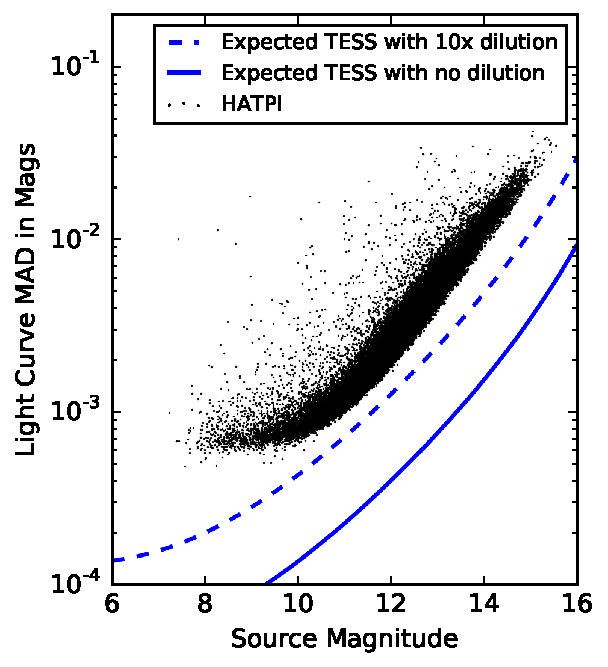
\includegraphics[width=1.05\textwidth]{figures/norefnoise_rms_vs_mag_binned30min_TESScomparison.pdf}
        %\caption{A subfigure}
        %\label{fig:sub3}
    \end{subfigure}
    \caption{Application of difference imaging to the field shown in the right 
    panel of Figure~\ref{fig:FieldComparison}.
    {\it Left}: The 2.2$^\circ$ region surrounding the cluster M\,25.
    {\it Middle:} Typical difference image. Variable stars are black 
    or white; saturated stars are masked; other artifacts are PSF residuals.
    {\it Right:} Variability (median absolute deviation) of HATPI light 
    curves, at 30 minute cadence, for thousands of stars in this crowded 
    field. The solid curve is \tess's expected performance, ignoring signal 
    dilution by blended stars~\citep{Sullivan_et_al_2015}. The dashed curve 
    accounts for dilution by a factor of 10.
    HATPI's light-collecting area is similar to that of \tess,
    and HATPI achieves a precision comparable to that expected from \tess.
    }
    \label{fig:hatpi_feasibile}
\end{figure}

\vspace{-0.3mm}
The \tess\ full-frame images of star clusters are a gold mine for
stellar astrophysics and exoplanetary science.  However the gold will
remain in the ground without a dedicated effort to solve the problem
of achieving high photometric precision in crowded images.  With
funding from the NESSF we will adapt our codes for difference
imaging to the {\it TESS} full-frame images.  We will make the light
curves available through MAST, and we will make the source code for
image subtraction, photometry, and detrending available on github. We
will also search the light curves of suitable stars for transiting
planets, which we intend to validate and follow up.  Through this
effort we can expect to quadruple the number of known transiting planets in
clusters, and provide a glimpse of the evolving physical and dynamical
properties of giant planets.


\vspace{-0.3mm}
\section{Relevance to NASA's Astrophysics \& Planetary Science Goals}
\vspace{-0.3mm}
Our proposal aims to discover and study planets around other stars, 
which is a goal of NASA's Astrophysics 
subdivision~\citep[][Ch.~4.4]{NASA_strategic_2014}. 
The analysis will be primarily enabled by \tess, an Astrophysics Explorer 
mission.
The effort will enhance \tess's science return because
\begin{itemize}
\item[A)] we will use a different reduction method from the mission's 
science team (difference imaging vs.~aperture photometry),
which will increase our photometric precision in crowded fields;
\vspace{-0.4mm}
%
\item[B)] we will focus our analysis and follow-up efforts near the 
galactic plane, which will be neglected by the mission's prioritization 
metrics~\citep{Stassun_et_al_2017}. 
%
\item[C)] we will perform high resolution ground-based photometric follow-up 
with the CHAT 0.7m to validate candidate transiting planets;
%
\item[D)] we will deliver our light curves to the MAST public archive, 
which will facilitate a wide range of other investigations. The \tess\ team 
has only committed to producing lightcurves for 200,000 stars amenable to 
transiting exoplanet detection, most of which will be far from the galactic 
plane~\citep{Stassun_et_al_2017}. 
\vspace{-0.4mm}
%
\
\end{itemize}

Our proposal also addresses topics solicited by the Planetary Science 
subdivision: one way to improve understanding of how exoplanet systems form 
and evolve is to observe them at known ages. 
By studying the sizes of transiting planets as a function of age, 
we could indirectly observe processes including photoevaporation and giant 
planet contraction.
By discovering hot Jupiters around young hosts, we could also
help distinguish between hot Jupiter formation scenarios, since the timescales 
for some variants of high-eccentricity migration are longer than those for 
disk migration~\citep[\textit{e.g.},][]{dawson_origins_2018}.
Another way to help distinguish between hot Jupiter formation channels would 
be measuring exoplanet (occurrence, period, age) or (occurrence, eccentricity, 
age) relations. For such analysis efforts to be convincing, we must first 
expand the sample of giant planets with known ages.




\vspace{-0.3mm}
\section{Timeline \& Expected Publications}
\vspace{-0.3mm}
\begin{figure}[!h]
    \centering
    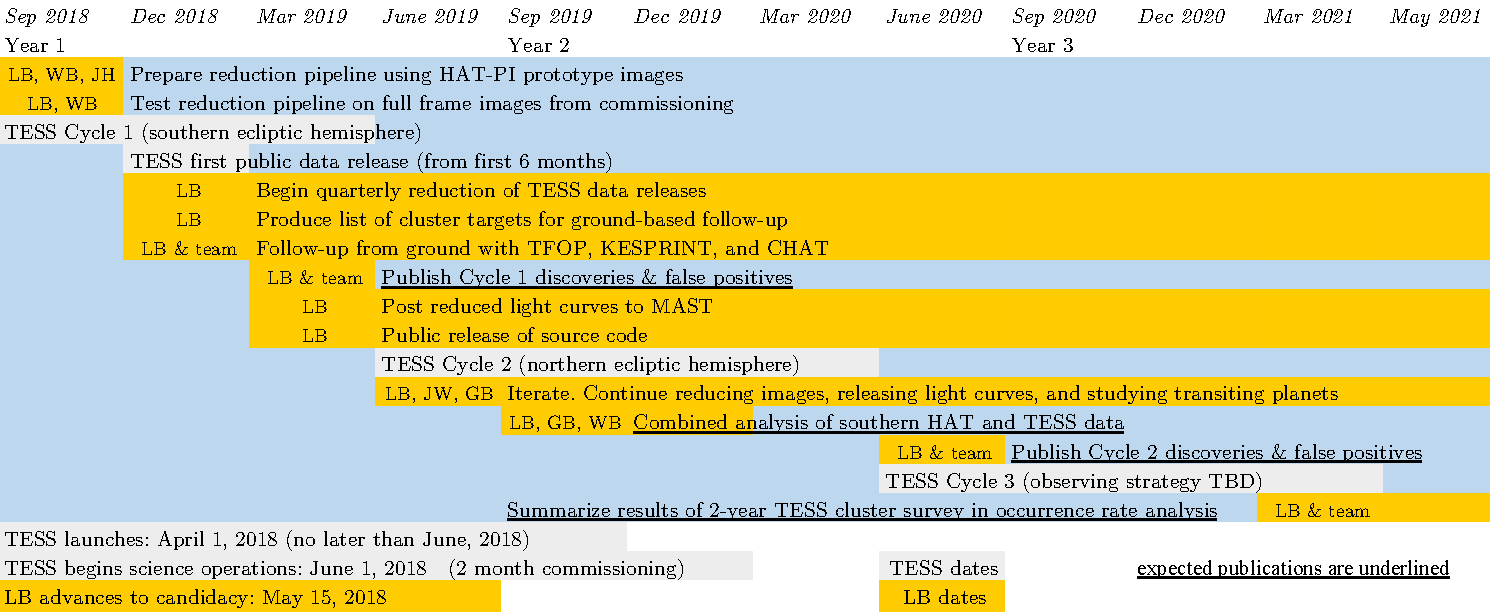
\includegraphics[width=\textwidth]{figures/work_plan_crop.pdf}
    \caption{
    Project timeline. Colors correspond to the planned times of each task.
    Team members~---~LB: Luke Bouma, JW: Joshua Winn, GB: G\'asp\'ar 
    Bakos, JH: Joel Hartman, WB: Waqas Bhatti.
    \label{fig:work_plan}}
\end{figure}

A timeline listing our major expected milestones, as well as those of the 
\tess\ project, is shown in Figure~\ref{fig:work_plan}.
Once our \tess\ data reduction pipeline has been heavily automated, we will 
begin a second component of the project: jointly analyzing the HAT and \tess\ 
lightcurves in the southern sky.
Extending the observing baseline for these targets beyond the expected 
$\approx\!28\,{\rm days}$ of \tess\ photometry will improve our sensitivity 
to longer period planets.

At least four publications are expected from the three-year effort.
Their respective topics will be:
1) \tess\ Cycle~1 planet discovery paper;
2) combined southern-sky HAT and \tess\ planet discovery paper;
3) \tess\ Cycle~2 planet discovery paper;
4) injection-recovery analysis of cluster survey from Cycles~1~\&~2, with 
occurrence rate estimate over as many ages as possible.



\vspace{-0.3mm}
\section{Robustness of Research Plan to Anticipated Setbacks}
\vspace{-0.3mm}

If the \tess\ mission performs as expected, the technical challenges of this 
project are surmountable: we showed in 
Figures~\ref{fig:FieldComparison}~\&~\ref{fig:hatpi_feasibile} that we
can reduce images analogous to the \tess\ full-frames images, in crowded 
fields with heavy blending.
Beyond applying photometric and centroid tests to \tess\ data, we will 
vet for astrophysical false positives by performing higher resolution 
follow-up photometry with the CHAT 0.7m ($\approx 0.7''/{\rm px}$ over a 
$0.4^\circ\times 0.4^\circ$ 
field of view). This will be especially important for determining which stars 
are the planet-hosts in crowded regions.

If \tess' photometric precision is worse than expected, our project 
will still have a high impact; our planet yield estimates are not strongly 
dependent on low-SNR detections, and so we can afford a somewhat lower
photometric precision.
Relatedly, young stars are more variable than old stars, and so their light 
curves will be noisier over transit timescales than assumed
by~\citet{Sullivan_et_al_2015}.
For young stars in clusters, simultaneously fitting for dips and a 
quadratic continuum during the transit search can help recover any losses in 
detection efficiency~\citep{rizzuto_zodiacal_2017}.

Finally, there is a community-oriented question: the \tess\ team, and other 
teams interested in cluster planets, will detect some planets in clusters 
before us.
This will at most marginally affect our work's impact: our publicly-released 
light curves will still be useful for broad community science, and they will 
still achieve higher photometric precision than simple aperture photometry.
Our approach will help maximize the overall number of detected planets in 
clusters, and so no matter what will be valuable for systematically studying 
planet occurrence as a function of age.

\vspace{.3cm}

%%%%%%%%%%%%%%%%%%%%%%%%%%%
%%%%%%%%%%%%%%%%%%%%%%%%%%%


% References {\it are included} when considering the proposal 4 page limit.
%\begingroup
%    \setlength{\bibsep}{10pt}
%    \linespread{1}\selectfont
%    \nobibliography{bibliography}{}
%\endgroup
%\newpage
%\newpage
\noindent
{ \tiny
\bibliography{bibliography}{}
}
%\bibliographystyle{aasjournal}

%%%%%%%%%%%%%%%%%%%%%%%%%%%
%%%%% End of document %%%%%
%%%%%%%%%%%%%%%%%%%%%%%%%%%

\end{document}

